% Chapter Template

\chapter{Conclusion} % Main chapter title

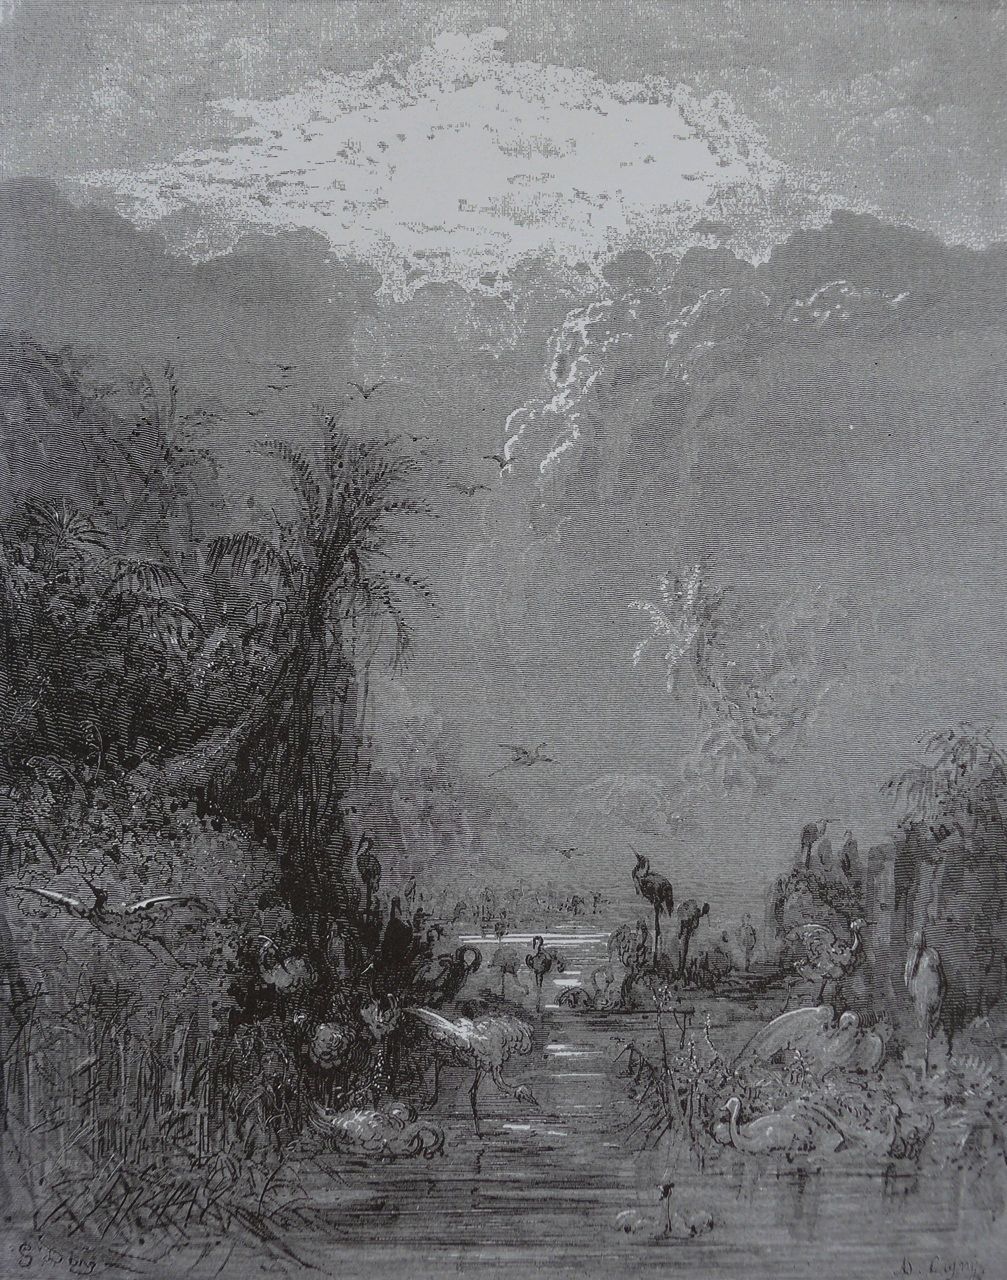
\includegraphics[width=\linewidth,trim={0 4cm 0 15cm},clip]{Paradise_Lost_33}

\label{Chapter 8} % Change X to a consecutive number; for referencing this chapter elsewhere, use \ref{ChapterX}

This final chapter will begin by going over the project as a whole and what was achieved during it. Then it will provide an evaluation against the motivation of the project to determine if what was achieved was in line with the aims. Finally, the research questions will be answered.

%----------------------------------------------------------------------------------------
%	SECTION 1
%----------------------------------------------------------------------------------------

\section{Paradise Restored?}

\label{Ch8 Sec1}

%----------------------------------------------------------------------------------------
%	SECTION 2
%----------------------------------------------------------------------------------------

\section{Research Question Answers}

\label{Ch9 Sec2}

\textit{What are the missing or non-functional sub-systems that the MEGA65 requires to be implemented?}\\
The missing and/or non-functional sub-systems of the MEGA65 are:
\begin{itemize}
\item{Save state Saving and Loading}
\item{Secure mode Saving and Loading}
\item{Secure mode ACCEPT and REJECT Implementation}
\item{SD card Read Protection}
\item{CPU Lock Protection}
\item{Matrix mode Key Scanning}
\item{SDXC Compatability}
\end{itemize}

\textit{How can these sub-systems be implemented?}\\
These sub-systems can be implemented as follows:
\begin{itemize}
\item{balh}
\end{itemize}

\textit{How can the simplicity, understandability and hence, the security of these sub-systems be maximised?}\\
By implementing the sub-systems in accordance with the UNIX philosophy of "Do one thing and do it well.", it was possible to create highly understandable and secure units that are able to make up the whole that is the MEGA65
\\
\textit{How can the complete MEGA65 architecture be physically prototyped on the bench?}\\
The complete architecture of the MEGA65 was prototyped via an FPGA. This FPGA contained the all of the MEGA65 architecture and was supplemented by 3rd party hardware, such as the modem.
\\
\textit{How can the secure compartmentalisation's architecture planned for the MEGA65 be realised?}\\
blah
